\documentclass[usenames,dvipsnames]{beamer}
\usetheme{Singapore}
\usepackage[utf8]{inputenc}
\usepackage[dvipsnames]{xcolor}

\title{Analyze of architecture of presentation layer in microservices applications}
\subtitle{with microfrontend}
\author{Aleksander Orchowski}
\institute{University of Zielona Góra}
\date{Promoter: Dr Grzegorz Bazydło}

\setbeamertemplate{footline}
{
	\leavevmode%
	\hbox{%
		\begin{beamercolorbox}[wd=.2\paperwidth,ht=2.25ex,dp=1ex,center]{author in head/foot}%
			\usebeamerfont{author in head/foot}\insertshortauthor
		\end{beamercolorbox}%
		\begin{beamercolorbox}[wd=.70\paperwidth,ht=2.25ex,dp=1ex,center]{title in head/foot}%
			\usebeamerfont{title in head/foot}\insertshorttitle
		\end{beamercolorbox}%
		\begin{beamercolorbox}[wd=.1\paperwidth,ht=2.25ex,dp=1ex,right]{date in head/foot}%
			\insertframenumber{} / \inserttotalframenumber\hspace*{2ex} 
	\end{beamercolorbox}}%
	\vskip0pt%
}
\makeatother

\begin{document}
\begin{frame}
	\titlepage
\end{frame}


\subsection{Why do we want to decouple everything?}
\begin{frame}
\frametitle{Why do we want to decouple everything?}\pause
Or in other words what's wrong with monolithic systems?\pause
\begin{itemize}
	\item We can't understand a big amount of code\pause
	\item So, we can't easily add new features\pause
	\item They are complex\pause
	\item One codebase can be developed effectively by 100 people?\pause
	\item Let's skip performance and scalability
\end{itemize}
Always? It depends. The good architecture also relates to monoliths.
\end{frame}

\begin{frame}
One of the biggest advantages of distributed systems is that knowledge is
also distributed through teams. They can focus on a single part of
business requirements.

Also, It's possible to easily \textbf{replace} each part.
\end{frame}

\begin{frame}
But, everything is loosely coupled...
\end{frame}

\subsection{Architectuure!}
\begin{frame}
\frametitle{Architectuure!}
Do microservices solve your problems? ARE YOU SURE?
\begin{figure}
	\centering
	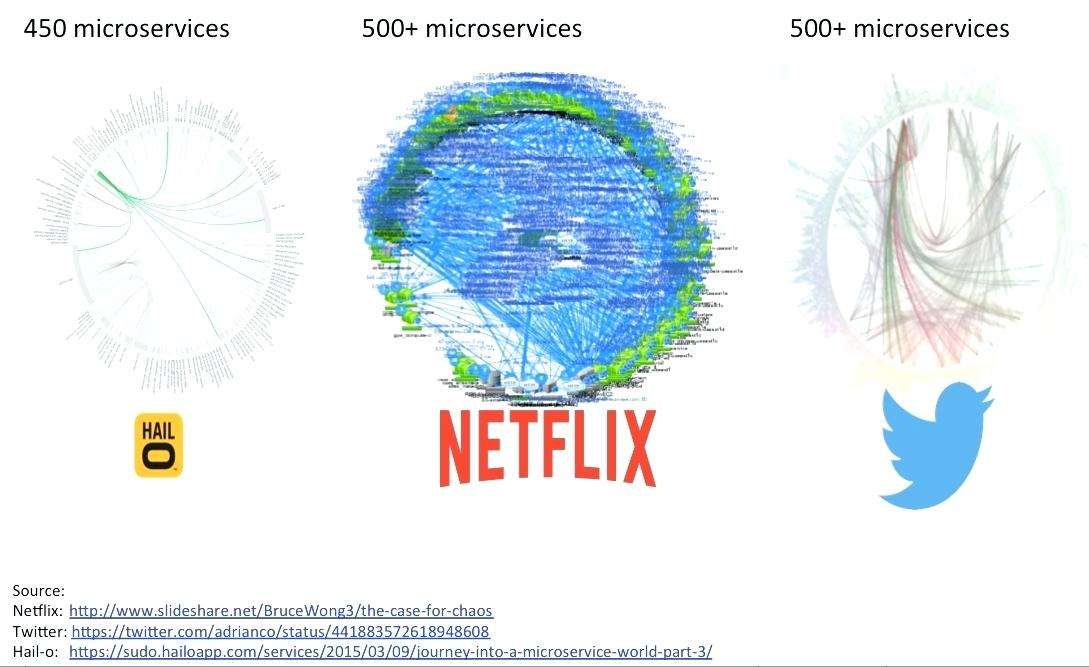
\includegraphics[width=1\linewidth]{pictures/exampleOfMicroservices}
	\label{fig:microservicesexamples}
\end{figure}


\end{frame}

\begin{frame}
\frametitle{For that - DevOps}
\begin{figure}
	\centering
	
\includegraphics[width=0.4\linewidth]{pictures/fenix.jpeg}
\end{figure}


\end{frame}




\begin{frame}
\frametitle{Okay... 500 Microservices but...}
\begin{figure}
Let's connect everything on UI...\pause
\end{figure}
\begin{figure}
	\centering
	
\includegraphics[width=0.7\linewidth]{pictures/killme}
	\label{fig:killme}
\end{figure}


\end{frame}



\section{Frontend that we know}
\begin{frame}
  \frametitle{Frontend that we know}
Now we are going to talk about approaches used at today's systems. \newline

I use the example of the blog app:
\begin{itemize}
	\item Service which manage users, authentication etc.
	\item Service for articles (listing, creating, editing, etc.)
	\item Frontend is SPA/SPA like
\end{itemize}
\end{frame}


\subsection{Monolith}

\begin{frame}
	\frametitle{Monolith}
	It's important to understand something about structure of application.
	So, we have one big block of code:
	\begin{figure}
		\centering
		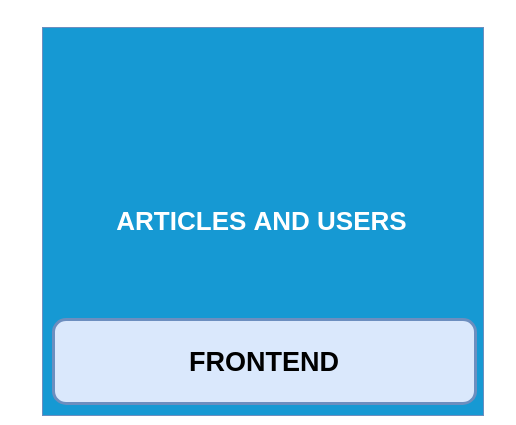
\includegraphics[width=0.6\linewidth]{pictures/monolit.png}		
		\label{fig:monolit}
	\end{figure}
\end{frame}

\begin{frame}
	\frametitle{Pros\&Cons}
	\begin{columns}[t]
		\column{0.5\linewidth}
			\textbf{\begin{center}
				+
			\end{center}}
		
		\begin{itemize}
			\item Everything at one place
			\item Probably - at one pull request we can add new feature 
			\item Deployed once with a frontend. We are sure that both layers work fine together
		\end{itemize}
		\pause
		
		\column{0.5\linewidth}
			\textbf{\begin{center}
				--
			\end{center}}
		
		\begin{itemize}
			\item Vertical scalability
			\item Complex inside
			\item A lot of legacy code can exist
			\item High entry threshold
		\end{itemize}
	
	\end{columns}
\end{frame}

\subsection{Microservices}

\begin{frame}
\frametitle{Microservices}
	\begin{figure}
		\centering
		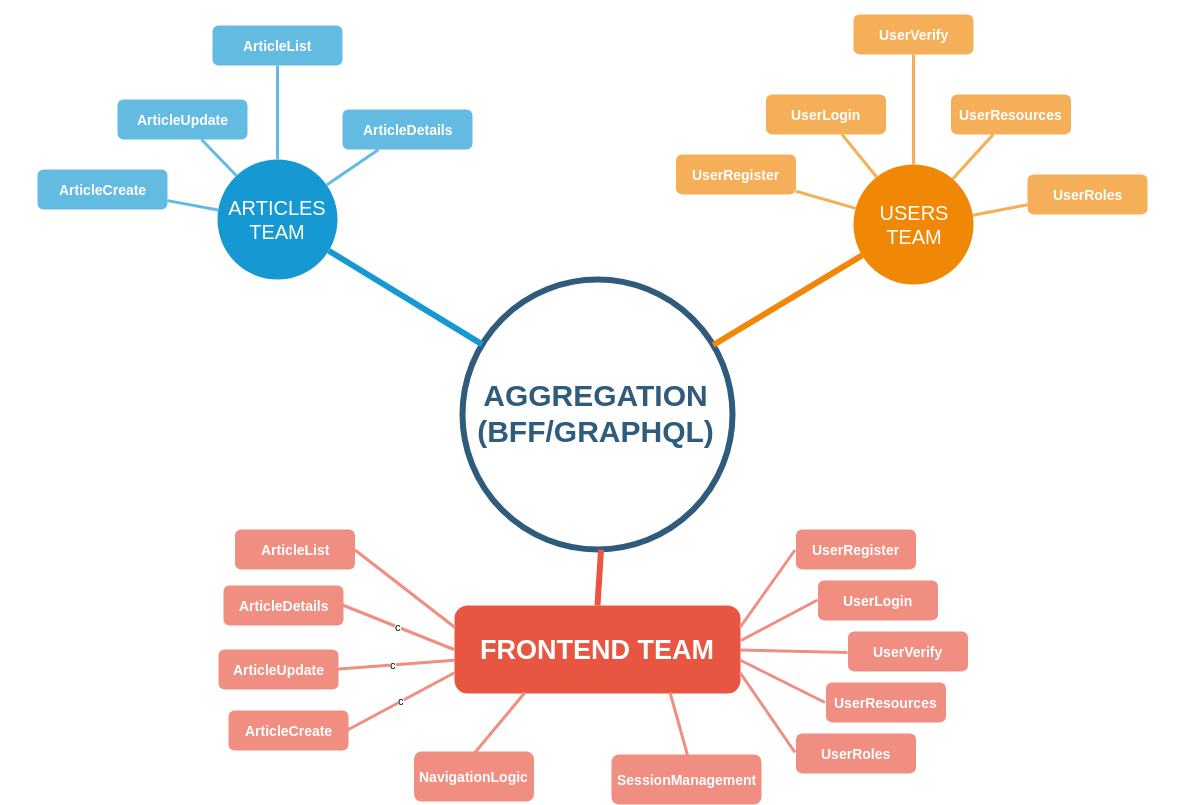
\includegraphics[width=0.8\linewidth]{pictures/microservices-knowledge.png}		
		\label{fig:microservices}
	\end{figure}
\end{frame}

\begin{frame}
\frametitle{Pros\&Cons}
\begin{columns}[t]
	\column{0.5\linewidth}
	\textbf{\begin{center}
			+
	\end{center}}
	
	\begin{itemize}
    	\item Working parallel \pause
		\item Many smaller codebases \pause
		\item This codebases are really small \pause
		\item Microservices are trendy now \pause
		\item We can use a lot of cool tools\pause
		\item We are skipping performance and scalability
	\end{itemize}\pause
	
	
	\column{0.5\linewidth}
	\textbf{\begin{center}
			--
	\end{center}}
	
	\begin{itemize}
		\item Many codebases - additional automation costs
		\item Integration needed (+ more testing etc.)
		\item Infrastructural costs
		\item Eventual consistency
		\item ...
		\item Just a lot of work more
	\end{itemize}
	
\end{columns}
\end{frame}




\section{Microfrontends}

\begin{frame}
\frametitle{Microfrontends}
	\begin{figure}
		\centering
		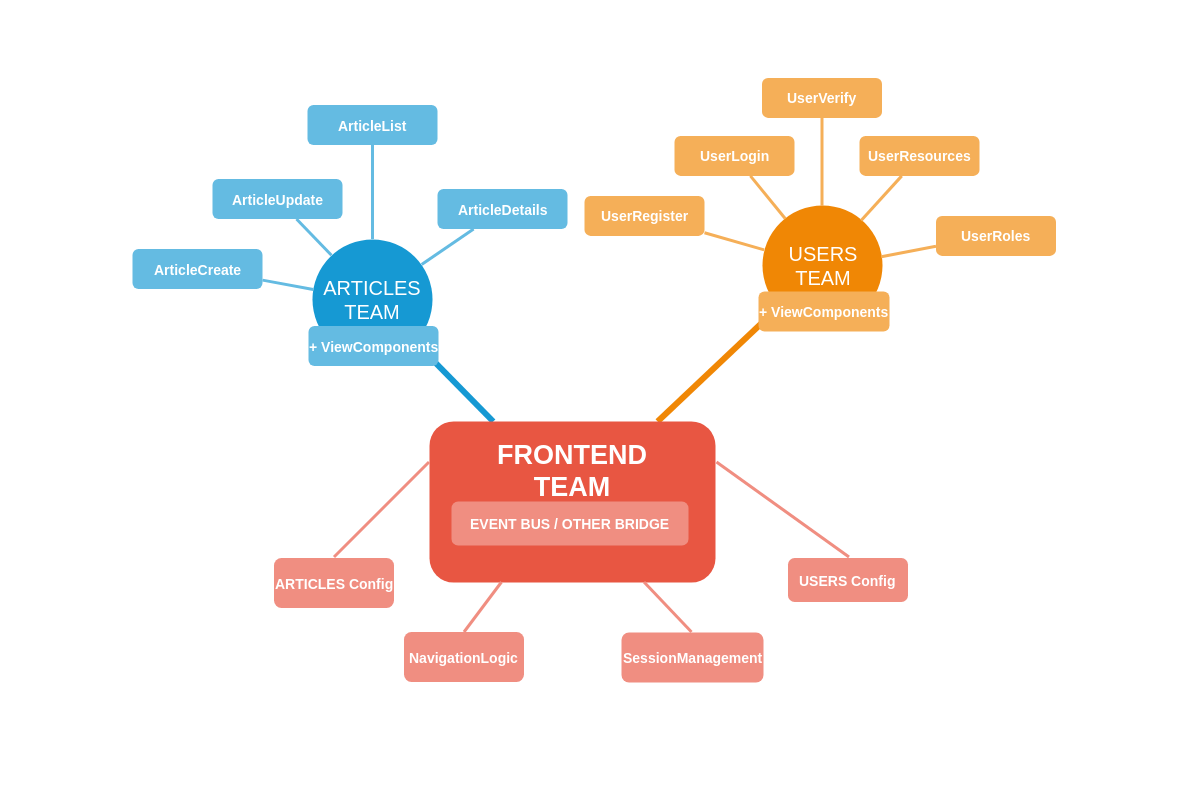
\includegraphics[width=0.9\linewidth]{pictures/microfrontends-knowledge.png}		
		\label{fig:microservices}
	\end{figure}
\end{frame}

\begin{frame}
\frametitle{Webcomponents}
Additional HTML tags defined in java script files, which can be shared between a lot of pages.
\begin{figure}
	\centering
	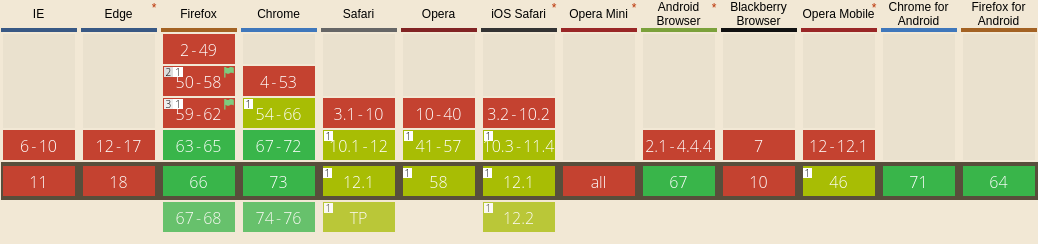
\includegraphics[width=1\linewidth]{pictures/webcomponents-support.png}		
	\label{fig:microservices}
\end{figure}
\end{frame}

\begin{frame}
\frametitle{Comparison}
\begin{figure}
	\centering
	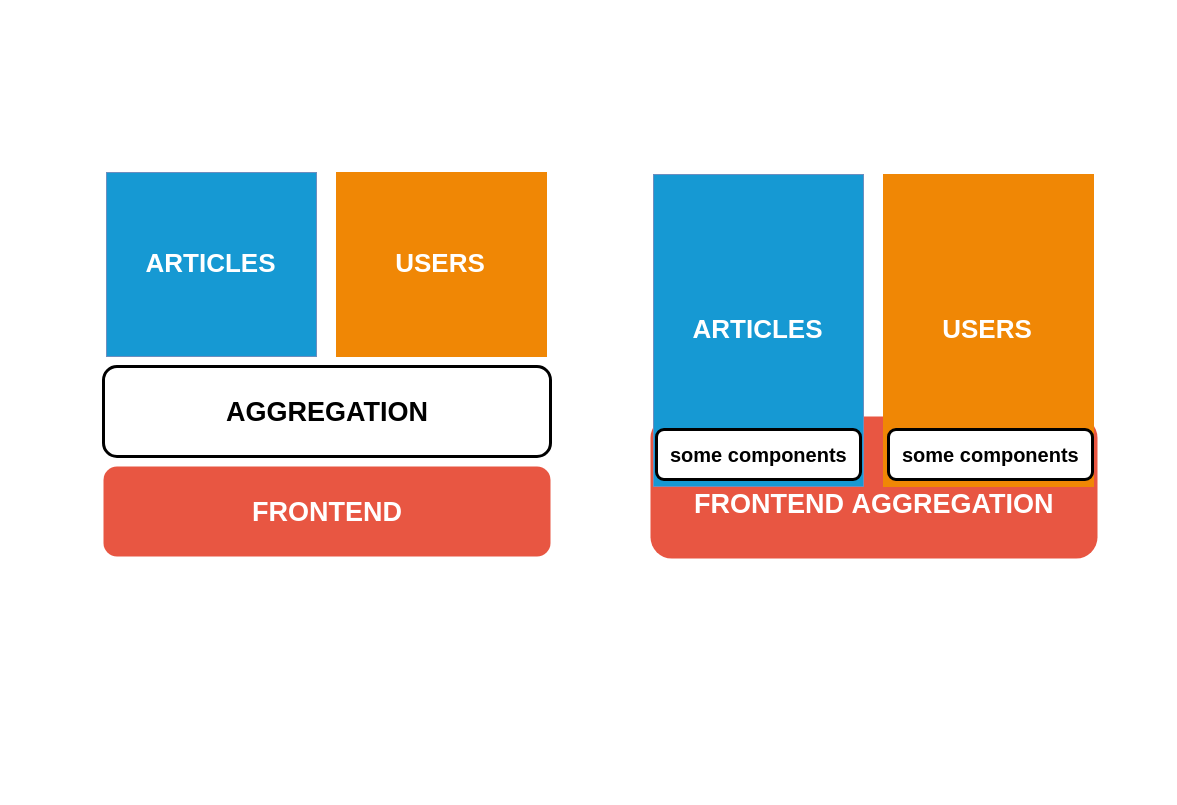
\includegraphics[width=0.9\linewidth]{pictures/microfrontends-vs-microservices.png}		
	\label{fig:vs}
\end{figure}
\end{frame}

\begin{frame}
	\frametitle{Multi-framework}
	\pause
	\begin{figure}
		\centering
		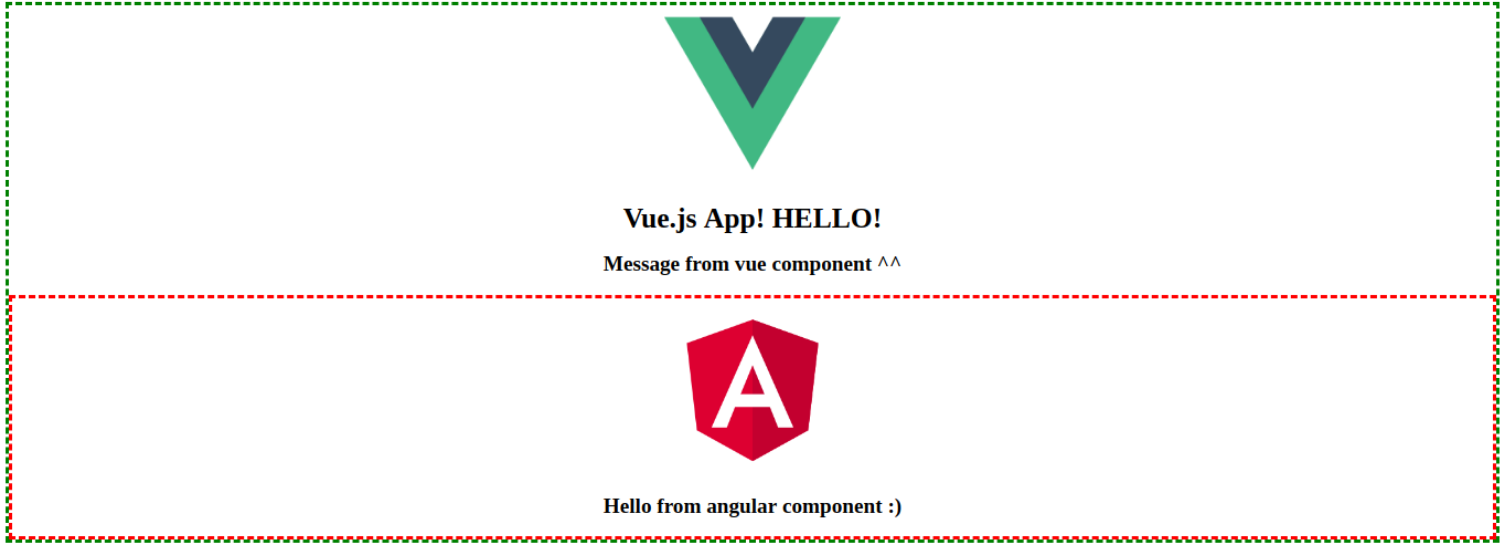
\includegraphics[width=1
		\linewidth]{pictures/angular-inside-vue}

		\label{fig:angular-inside-vue}
	\end{figure}
	
\end{frame}

\section{Diploma}
\begin{frame}[t]
\frametitle{Diploma work}
	\begin{columns}[t]
	\column{0.5\linewidth}
	\textbf{\begin{center}
			Project area
	\end{center}}
	\begin{itemize}
		\item Microfrontends \textcolor{ForestGreen}{100\%}
		\item Microservices + standard frontend \textcolor{ForestGreen}{100\%}
	\end{itemize}
	
	\column{0.5\linewidth}
		\textbf{\begin{center}
			Theory area
	\end{center}}
	\begin{itemize}
		\item Reading needed literature : \textcolor{ForestGreen}{70\%}
		\item Diagrams are prepared
	\end{itemize}
	\end{columns}
\end{frame}

\section{End}
\begin{frame}[t]
\frametitle{Questions?}
\end{frame}
%\section{Next}
%\begin{frame}
%\frametitle{Outline}
%\end{frame}
%
%
%\subsection{Subsection1}
%\begin{frame}
%\frametitle{Outline}
%\end{frame}
%
%
%\subsection{Subsection2}
%\begin{frame}
%\frametitle{Outline}
%\end{frame}

\end{document}